Existem diversas formas de se obter o modelo de um robô, tais como Denavit-Hartenberg clássico, Denavit-Hartenberg modificado e através das matrizes de transformação homogêneas de cada um dos \textit{frames} no robô. Nesse trabalho o método escolhido para se obter a expressão matemática foi Denavit-Hartenberg clássico. 

\subsection{Diagrama de arames}
O primeiro passo para a aplicação da técnica escolhida é fazer uma simplificação do manipulador robótico por meio da representação em diagrama de arames. Este deve ser feito com o robô em posição de \textit{home} conforme pode-se verificar na FIG. \ref{fig:home}.

\begin{figure}[h]
    \centering
    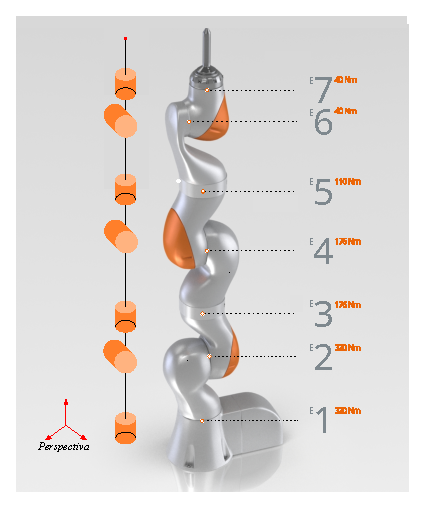
\includegraphics[width=0.45\textwidth]{Imagem/Arames.eps}
    \caption{Posição \textit{home} do manipulador.}
    \label{fig:home}
    Fonte: \citeauthor{KUKA3D}, 2020. (Desenho dos frames e indicação dos eixos e seus respectivos torques).
\end{figure}

\subsection{Atribuição de \ensuremath{z}}
Uma vez que o diagrama de arames foi definido então pode-se aplicar a convenção de Denavit-Hartenberg. Para determinar os frames do robô, deve-se atribuir os eixos $z_i$ nos eixos de atuação para cada junta $i+1$, sendo $i = 0,\;1,\;2,\dots,\;n-1$, em que $n$ é o número de juntas do manipulador. O eixo $z_n$, referente ao frame do \textit{end-effector} ou \textit{tool frame}, deve ser atribuído ao final. Após atribuir os eixos $z_i$, então pode-se identificar a origem dos frames $i$, em que $i=1,\;2,\;\dots,\;n-1$ adotando a seguinte regra: 

\begin{itemize}
    \item Se $z_{i-1}$ interceptar $z_i$, então a origem do frame $i$ deve ser posicionada na interseção.
    \item Se não, mas se existe uma perpendicular comum à $z_{i-1}$ e $z_i$, então a origem fica nessa reta perpendicular comum. 
    \item Se nenhuma das opções anteriores são verdadeiras, então $z_{i-1}$ e $z_i$ são paralelos e assim a origem do sistema de coordenadas deve ser posicionada de forma que o modelo fique mais simples. 
\end{itemize}

Para o robô aqui estudado, pôde-se adotar a primeira regra para todos os \textit{frames}. Isso porque $z_{i-1}$ e $z_i$ se interceptam para todo $i=1,\;2,\;\dots,\;n-1$.

\subsection{Atribuição de \ensuremath{x}}
Com as origens $o_i$ e os eixos $z_i$ determinados, estabelece-se os eixos $x_i$, para $i=1,\;2,\;\dots,\;n-1$, considerando a seguinte regra:

\begin{itemize}
    \item Se $z_{i-1}$ interceptar $z_i$, então $x_i$ deve ser posicionado na direção normal ao plano de $z_{i-1}$e $z_i$
    \item Se não, então determina-se $x_i$ na perpendicular comum de $z_{i-1}$e $z_i$ a partir da origem do \textit{frame} $i$.  
\end{itemize}

No KUKA LBR iiwa, para todo $i=1,\;2,\;\dots,\;n-1$, os eixos $x_i$ foram atribuídos conforme a primeira regra.

\subsection{Atribuição de \ensuremath{y}}
Os eixos $y_i$ foram escolhidos implicitamente de forma que todos os sistemas de coordenadas fossem dextrogiros, como requerido pelo método clássico de Denavit-Hartenberg. Portanto, optou-se por excluí-lo do diagrama da FIG. \ref{fig:frames} para deixar mais fácil a sua visualização e obtenção dos parâmetros dos links.

\subsection{Referência e End-effector}
Por fim, foram atribuídos os \textit{frames} $0$ e $n$. Para o \textbf{end-effector}, já que o robô não apresenta garra, repetiu-se o frame $6$, como instruído no método DH clássico. O \textit{frame} $i=0$ foi atribuído na base do robô. Embora a atribuição não seja a mais simples, visto que se sua origem fosse atribuída junto aos \textit{frames} 1 e 2 reduzir-se-ia uma translação, ela facilitará na comparação dos resultados com a simulação no RoboDK. A FIG. \ref{fig:frames} expõe a atribuição de \textit{frames} descrita.

\begin{figure}[ht]
    \centering
    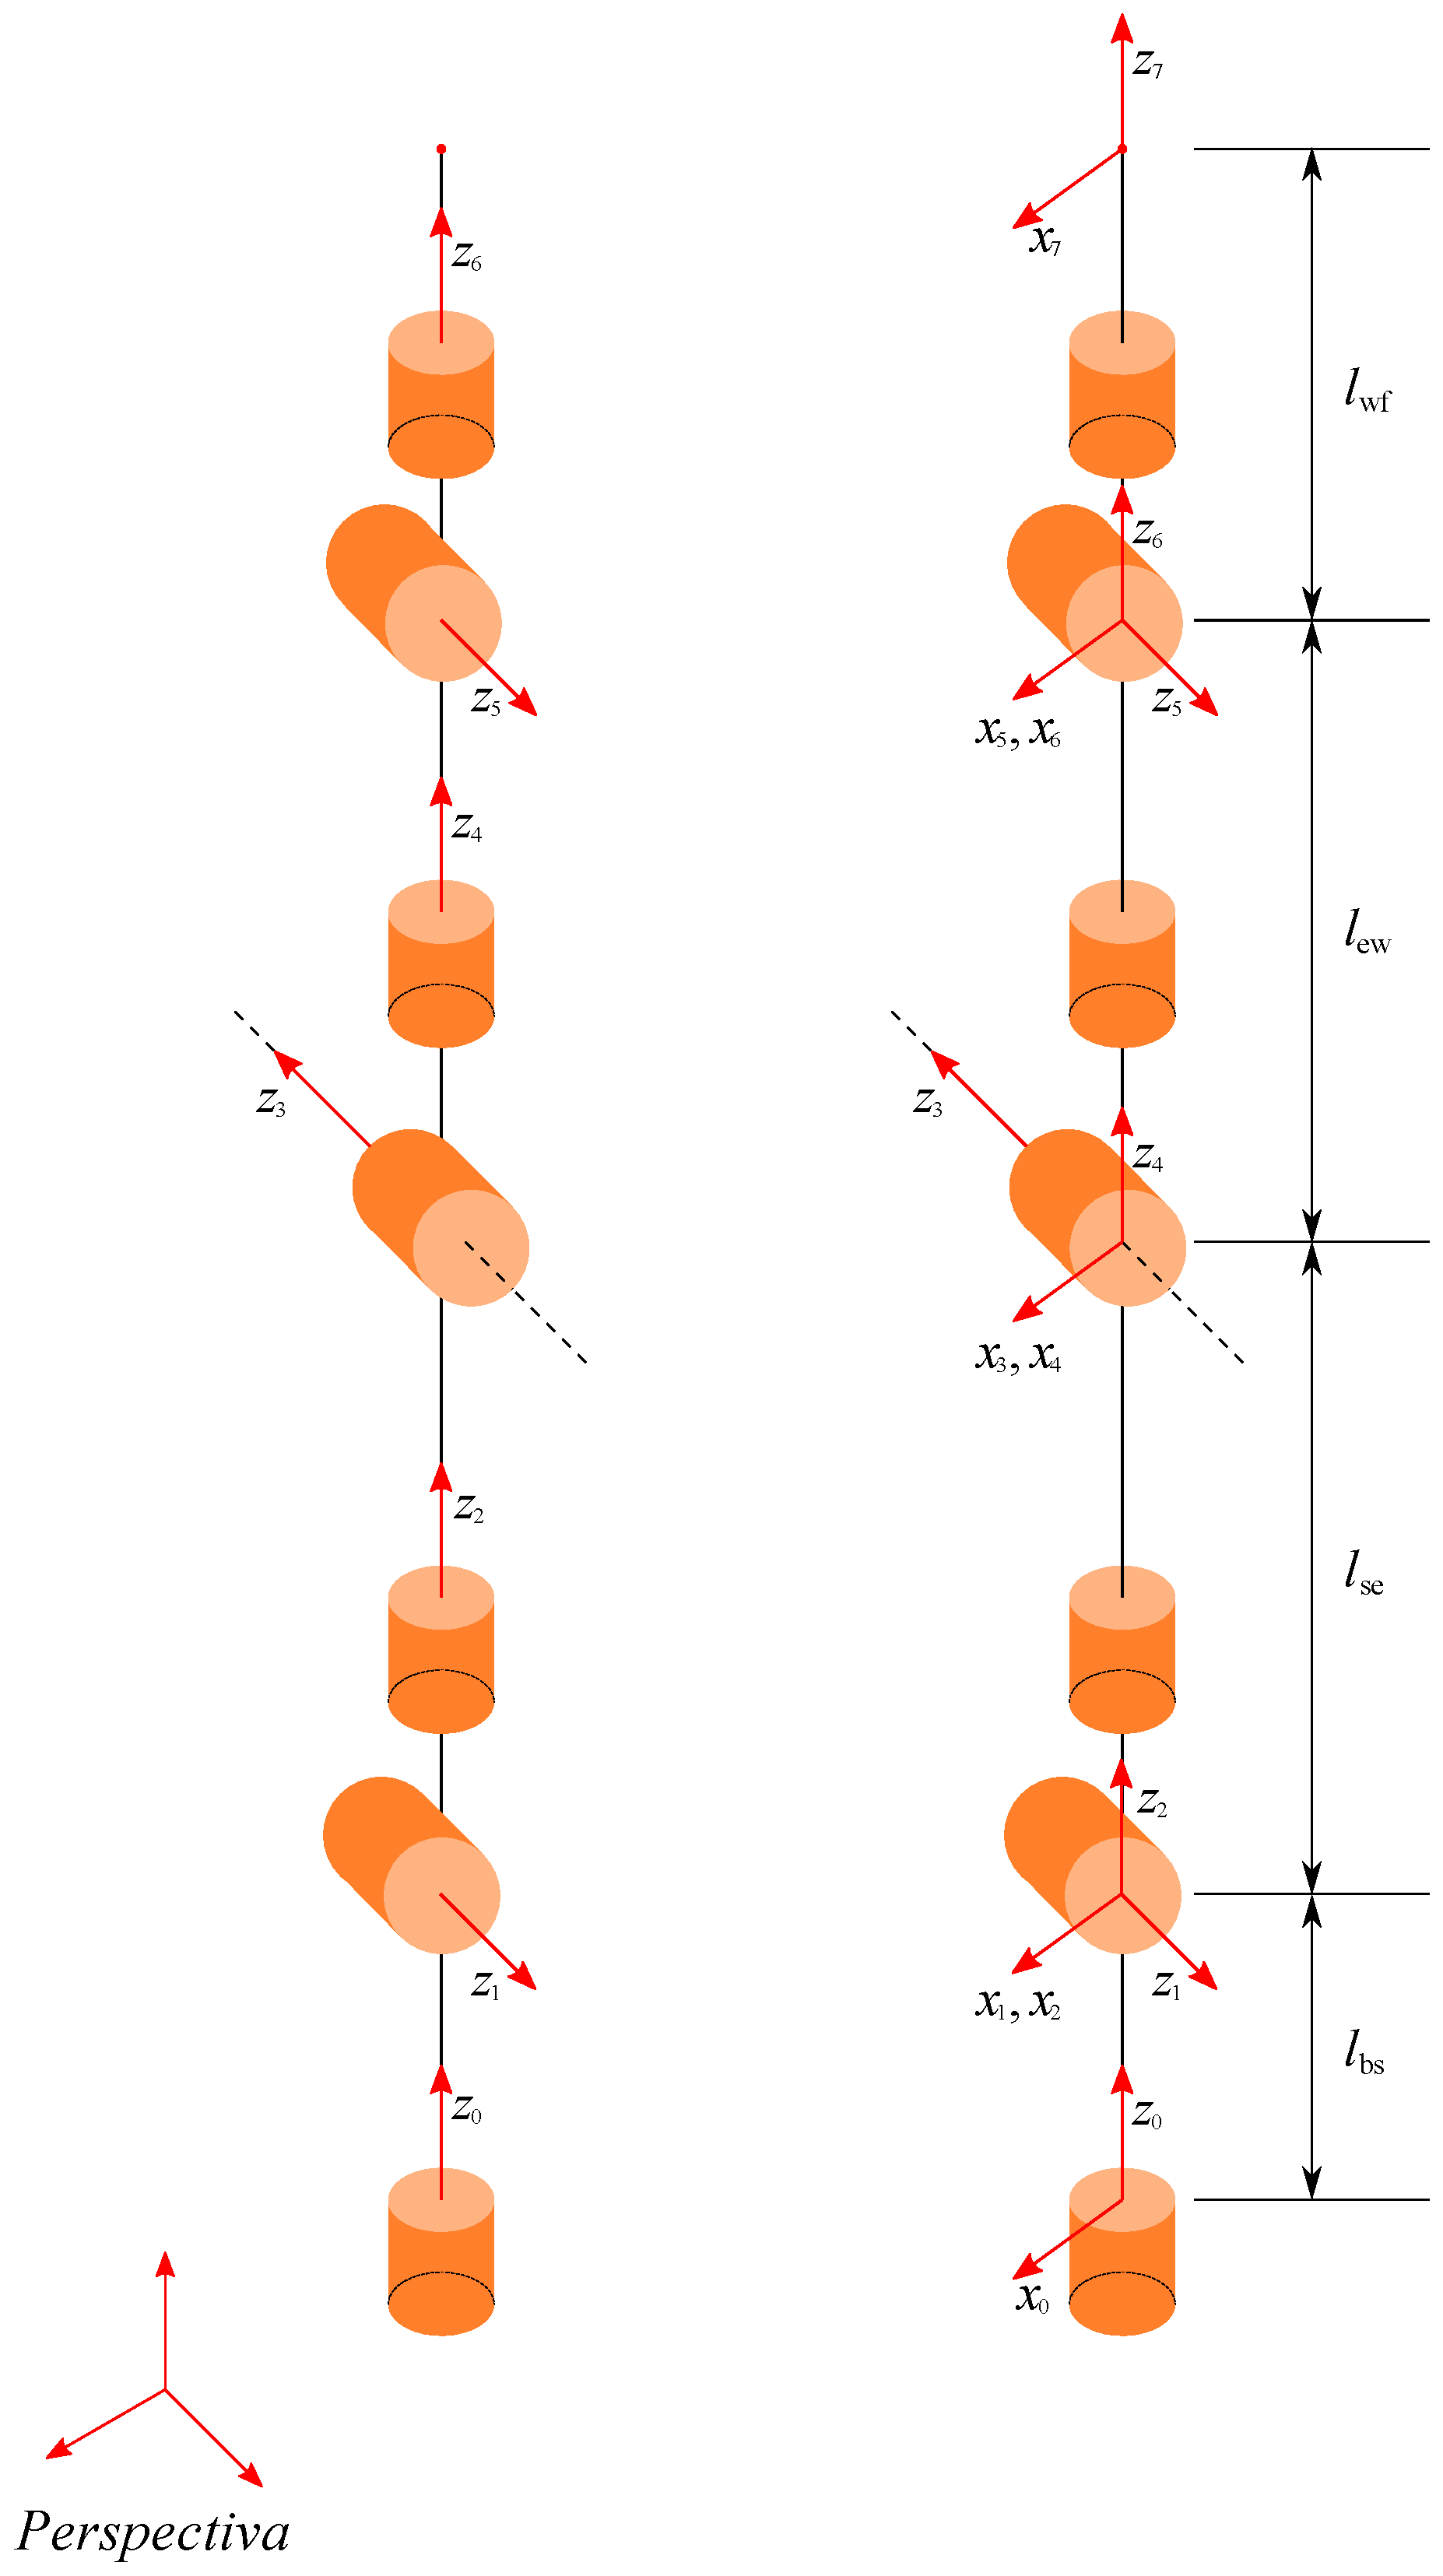
\includegraphics[width=0.45\textwidth]{Imagem/x.eps}
    \caption{Atribuição dos \textit{frames}}
    \label{fig:frames}
\end{figure}

\subsection{Tabela de Denavit-Hartenberg}

Após dispor todos os \textit{frames}, são determinados os parâmetros da tabela de Denavit-Hartenberg. Em cada uma de suas linhas é possível definir a matriz de transformação homogênea $A_i$ do \textit{frame} $i-1$ para o \textit{frame} $i$, fazendo  
\begin{align*}
  \setlength{\dashlinegap}{2pt}
    A_i
    &= \Rot_{z,\,\theta_i} \Trans_{z,\,d_i} \Trans_{x,\,a_i} \Rot_{x,\,\alpha_i} \\
    &=
    \left[ 
    \begin{array}{rrr;{2pt/2pt}c}
        c_{\theta_i} & -s_{\theta_i}c_{\alpha_i} & s_{\theta_i} s_{\alpha_i} & a_i c_{\theta_i} \\
        s_{\theta_i} & c_{\theta_i} c_{\alpha} & -c_{\theta_i} s_{\alpha} & a_i s_{\theta_i} \\
        0 & s_{\alpha_i} & c_{\alpha_i} & d_i \\
        \hdashline[2pt/2pt]
        0 & 0 & 0 & 1
    \end{array}
    \right]
\end{align*}
em que $a_i$ é a distância entre $z_{i-1}$ e $z_i$ medido ao longo de $x_i$; $\alpha_i$ o ângulo entre $z_{i-1}$ e $z_i$ mensurado no plano normal a $x_i$;  $d_i$ a distância perpendicular entre a origem $o_{i-1}$ e a interseção de $x_i$ com $z_{i-1}$, medido ao longo de $z_0$; $\theta_i$ o ângulo  entre $x_0$ e $x_1$ mensurado no plano normal a $z_0$.

Uma vez obtidas as matrizes $A_i$ para $i= 1,\;2,\;\dots,\;n$, então pode-se determinar a matriz de transformação $T$ do \textit{frame} $0$ para o \textit{frame} $n$ como
\begin{equation*}
    T_n^0 = \prod_{i=0}^n A_i
\end{equation*}

Para o braço robótico KUKA LBR iiwa, os parâmetros da tabela DH podem ser retirados da sua interpretação física da atribuição de \textit{frames} vista na FIG. \ref{fig:frames}. A TAB. \ref{tab:DH} expõe os valores obtidos. 

\begin{table}[h]
    \centering
    \caption{Parâmetros DH do KUKA LBR iiwa}
    \label{tab:DH}
    \begin{tabular}{crrrr}
    \toprule
        $i$ & $a_i$ & $\alpha_i$ & $d_i$ & $\theta_i$ \\
    \midrule
        1 & 0 & $-\pi/2$ & $\ell_\mathrm{bs}$ & $\theta_1^*$ \\
        2 & 0 &  $\pi/2$ &                  0 & $\theta_2^*$ \\
        3 & 0 &  $\pi/2$ & $\ell_\mathrm{se}$ & $\theta_3^*$ \\
        4 & 0 & $-\pi/2$ &                  0 & $\theta_4^*$ \\
        5 & 0 & $-\pi/2$ & $\ell_\mathrm{ew}$ & $\theta_5^*$ \\
        6 & 0 &  $\pi/2$ &                  0 & $\theta_6^*$ \\
        7 & 0 &        0 & $\ell_\mathrm{wf}$ & $\theta_7^*$ \\
    \bottomrule
    \end{tabular}
    
O $^*$ indica que é variável.
\end{table}

Para o link 1, segue $a_1 = 0$, $\alpha_1 = -\pi/2$, $d_1=\ell_\mathrm{bs}$ e $\theta_1$ sendo a variável, então
\begin{align*}
    A_1 
    &=
    \left[ 
    \begin{array}{rrr;{2pt/2pt}c}
        c_{\theta_1} & 0 & -s_{\theta_1} & 0 \\
        s_{\theta_1} & 0 &  c_{\theta_1} & 0 \\
        0 & -1 & 0 & \ell_\mathrm{bs} \\
        \hdashline[2pt/2pt]
        0 & 0 & 0 & 1
    \end{array}
    \right]
\end{align*}
Para o link 2, segue $a_2 = 0$, $\alpha_2 = \pi/2$, $d_2=0$ e $\theta_2$ sendo a variável, então
\begin{align*}
    A_2 &=
    \left[ 
    \begin{array}{rrr;{2pt/2pt}c}
        c_{\theta_2} & 0 &  s_{\theta_2} & 0 \\
        s_{\theta_2} & 0 & -c_{\theta_2} & 0 \\
        0 & 1 & 0 &  0 \\
        \hdashline[2pt/2pt]
        0 & 0 & 0 & 1
    \end{array}
    \right]
\end{align*}
Para o link 3, segue $a_3 = 0$, $\alpha_3 = \pi/2$, $d_3=\ell_\mathrm{se}$ e $\theta_3$ sendo a variável, então
\begin{align*}
    A_3 &=
    \left[ 
    \begin{array}{rrr;{2pt/2pt}c}
        c_{\theta_3} & 0 &  s_{\theta_3} & 0 \\
        s_{\theta_3} & 0 & -c_{\theta_3} & 0 \\
        0 & 1 & 0 &  \ell_\mathrm{se} \\
        \hdashline[2pt/2pt]
        0 & 0 & 0 & 1
    \end{array}
    \right]
\end{align*}
Para o link 4, segue $a_4 = 0$, $\alpha_4 = -\pi/2$, $d_4=0$ e $\theta_4$ sendo a variável, então
\begin{align*}
    A_4 
    &=
    \left[ 
    \begin{array}{rrr;{2pt/2pt}c}
        c_{\theta_4} & 0 & -s_{\theta_4} & 0 \\
        s_{\theta_4} & 0 &  c_{\theta_4} & 0 \\
        0 & -1 & 0 & 0 \\
        \hdashline[2pt/2pt]
        0 & 0 & 0 & 1
    \end{array}
    \right]
\end{align*}

Para o link 5, segue $a_5 = 0$, $\alpha_5 = -\pi/2$, $d_5=\ell_\mathrm{ew}$ e $\theta_5$ sendo a variável, então
\begin{align*}
    A_5 &=
    \left[ 
    \begin{array}{rrr;{2pt/2pt}c}
        c_{\theta_5} & 0 & -s_{\theta_5} & 0 \\
        s_{\theta_5} & 0 &  c_{\theta_5} & 0 \\
        0 & -1 & 0 &  \ell_\mathrm{ew} \\
        \hdashline[2pt/2pt]
        0 & 0 & 0 & 1
    \end{array}
    \right]
\end{align*}
Para o link 6, segue $a_6 = 0$, $\alpha_6 = \pi/2$, $d_6=0$ e $\theta_6$ sendo a variável, então
\begin{align*}
    A_6 &=
    \left[ 
    \begin{array}{rrr;{2pt/2pt}c}
        c_{\theta_6} & 0 &  s_{\theta_6} & 0 \\
        s_{\theta_6} & 0 & -c_{\theta_6} & 0 \\
        0 & 1 & 0 &  0 \\
        \hdashline[2pt/2pt]
        0 & 0 & 0 & 1
    \end{array}
    \right]
\end{align*}
Para o link 7, $a_7 = 0$, $\alpha_7 = 0$, $d_7=\ell_\mathrm{wf}$ e sendo $\theta_7$ a variável, segue
    \begin{align*}
        A_7 =
        \left[ 
    \begin{array}{rrr;{2pt/2pt}c}
        c_{\theta_7} & -s_{\theta_7} & 0 & 0 \\
        s_{\theta_7} &  c_{\theta_7} & 0 & 0 \\
        0 & 0 & 1 & \ell_\mathrm{wf} \\
        \hdashline[2pt/2pt]
        0 & 0 & 0 & 1
    \end{array}
    \right]
    \end{align*}
    Por fim, a matriz de transformação homogênea do \textit{frame} 7 para o \textit{frame} 0 é encontrada fazendo
    \begin{equation}
        T_7^0 = A_1 A_2 A_3 A_4 A_5 A_6 A_7
    \end{equation}
uma multiplicação de 7 matrizes $4\times4$ de variáveis reais. A solução dessa multiplicação, matriz de transformação $T_7^0$, pode ser verificada no Apêndice \ref{apend:MatrizT}, para qual foram adotadas as dimensões do KUKA LBR iiwa 14 820
\begin{alignat*}{3}
\ell_\mathrm{bs} &= \SI{360}{mm}, \quad& \ell_\mathrm{se} &= \SI{420}{mm}, \\
\ell_\mathrm{ew} &= \SI{400}{mm}, \quad & \ell_\mathrm{wf} &= \SI{90}{mm}.
\end{alignat*}

A matriz foi obtida via simulação computacional, realizada por meio de um código em \texttt{Python 3}, exposto no Apêndice \ref{apend:memoria_calculo}.